\chapter{Semantic Segmentation}
%



\section{Overview of our approach}
We train the most popular models for semantic segmentation for this highly diverse dataset. 
We train and test the networks on 2D slices of the rat brain MRI images. 
The trained networks input is an image slice of the MRI image and the output from the trained network is the segmentation mask. 
We start with 2D slices because it makes the networks much easier to train when compared to a 3D model as well as it uses much less memory. 
Using a 3D model though it is able to learn information along the slice direction as well. 
This information could be useful when learning semantic segmentation as the segmented regions are 3D in real life not 2D. 
Using the 3D volumes though requires a lot more time and memory to train. 
We mainly utilize dice coefficient loss in order to train the model.

\section{Deep Convolutional Neural Networks}
    We divide up the data into train and validation/test groups in order to prevent overfitting in our model. 
    The validation data is just used to visually make sure that our model is training correctly.  

\section{Convolutional Neural Network Architecture}
    We explore several convolutional neural networks in this paper, mainly focusing on U-net and dilation networks. 
    We choose to implement U-net and dilation networks because they were previously shown to be the most successful for the task of semantic segmentation while having their own benefits \cite{DBLP:journals/corr/LongSD14}, \cite{DBLP:journals/corr/RonnebergerFB15}, \cite{Yu2016MultiScaleCA}. 
    U-net is one of the most popular networks used for medical images and provides excellent results. 
    Dilation networks or networks with dilated convolutions also have excellent results for the task of semantic segmentation and is widely used. 

\subsection{U-net}
%
The U-net architecture has been very successful in semantic segmentation. 
U-net works very well because it extends the idea of fully convolutional networks like pooling and convolution layers to upsampling and deconvolutional layers \cite{DBLP:journals/corr/RonnebergerFB15}. 
U-net utilizes downsampling layers to leads to larger receptive field sizes \cite{DBLP:journals/corr/LongSD14}. 
The receptive field size is important because it determines where the network will look and so it is important to ensure that the receptive field size covers the relevant regions \cite{NIPS2016_6203}.
After the image is downsampled it is them upsampled back to its original size for the task it is learning.
In the case of semantic segmentation, the output of the model is required to be the same size as the input so that every pixel can have a probability associated with it.
The reason that U-net is so successful is the skip connections between the downsampled part and upsampled part of the network.
There is a skip connection from one layer of the downsampled network to the corresponding upsampled layer in the network so the first downsampling part is skip connectioned to the last upsampling layer. 
They help to not only preserve the shallow data that was lost in the downsampling, but keep the deep, semantic information to help training significantly \cite{DBLP:journals/corr/LongSD14}.

U-net has a base architecture shown in figure ~\ref{fig_Unet}. 
It is made up of four downsampling and four upsamplings layers with two convolutional layers in between. 
The reason that we have the upsampling layers is because we need the output to be a segmentation map of every pixel in the input.
We use deconvolution layers in order to upsample back to the original image size. 
The network also doubles the amount of features every time the network downsamples and halves the number of features every time it upsamples. 
This allows the network to be able to learn more robust contextual information by being able to use more combinations of the features from the previous layer, but also keep the important features as the model upsamples \cite{DBLP:journals/corr/RonnebergerFB15}. 
The input of the architecture is the image size in this case 256x256x3, but can be any image size as long as it is large enough to go through the downsampling layers.
For RGB images usually all three of those slices are put into the model for it to learn but with MRI images they are grayscale images and so only one slice is needed. 
The total amount of parameters in U-net is around 7 million. 
The number of parameters is important because that determines how well a model learns. 
A model with more parameters will take longer to train but will be able to learn more complex connections. 
Too many parameters though also isn't the best as your model will just learn the training dataset and won't be able to generalize well. 

\begin{figure}[tbh]
\centering
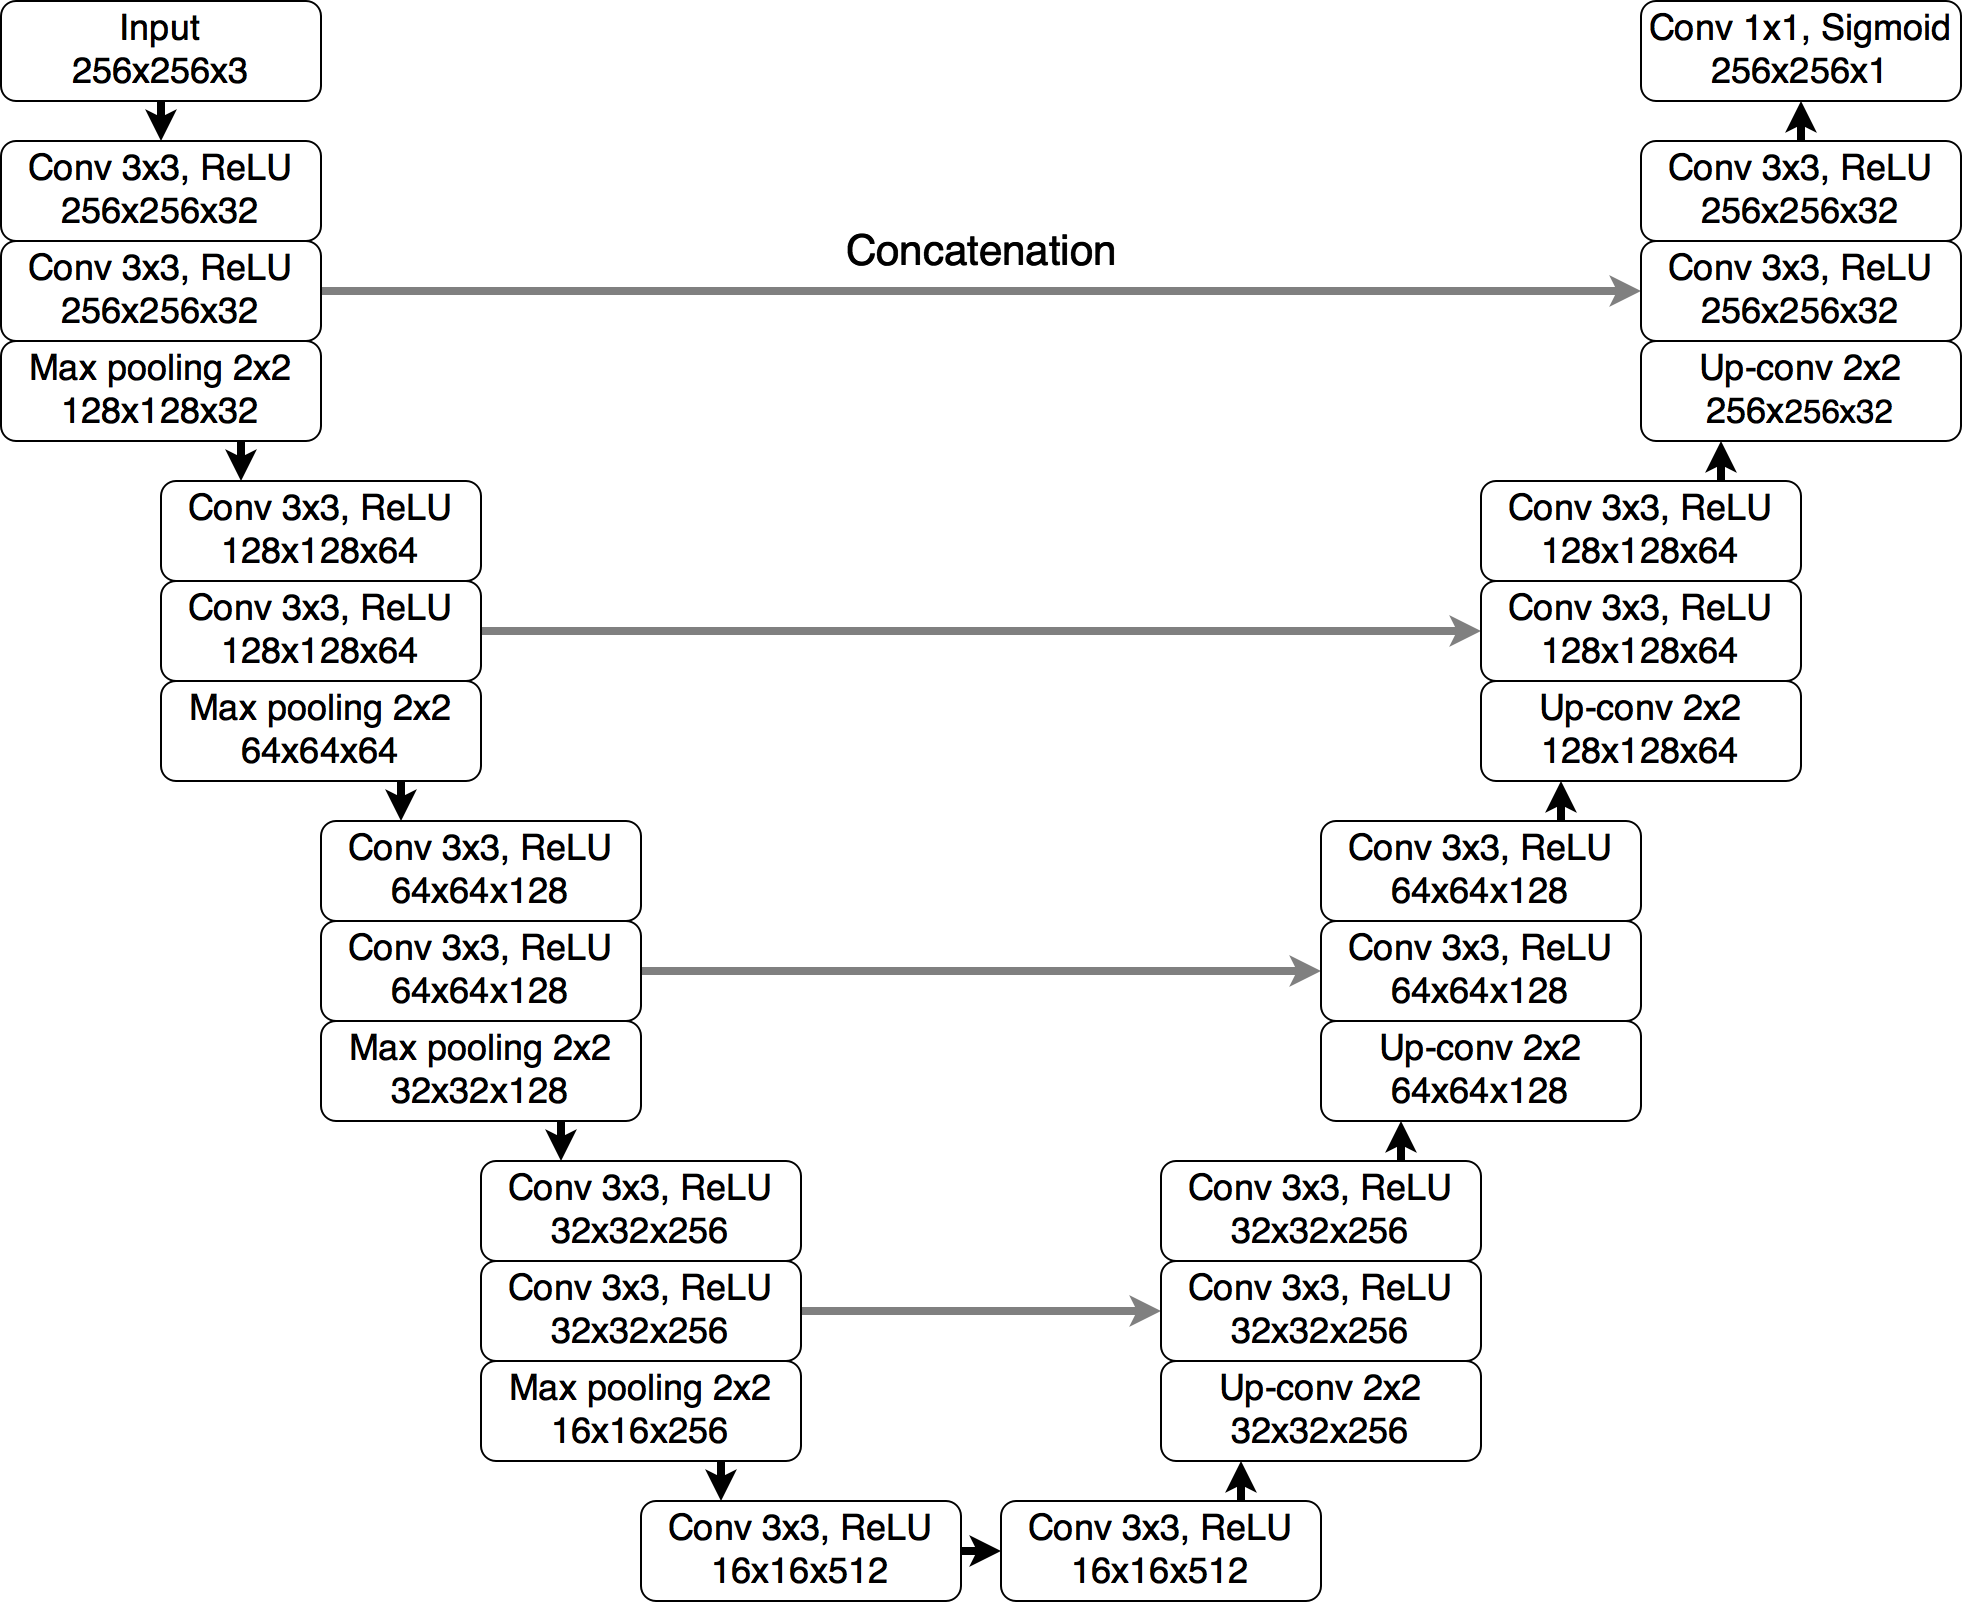
\includegraphics[width=\textwidth]{Unet_Architecture.png}
% where an .eps filename suffix will be assumed under latex,
% and a .pdf suffix will be assumed for pdflatex
\caption{Unet base architecture with input image 256x256x3. Each black arrow represents a pooling layer when pointing down or an unsampling layer when pointing up. The skip connections are represented by gray arrows or concatenation layers between the corresponding layers. The filter size is shown as the third dimension in the image size of each block except for the input layer where it corresponds to the image input. There is also batch normalization after each convolution layer.}
\label{fig_Unet}
\end{figure}

\subsection{Dilated Convolutions}
Dilated or atrous convolutions are another successful way where semantic segmentation has been implemented. 
Dilated convolutions are utilized because in order for semantic segmentation to be successful, one needs contextual information, as explained before dilated convolutions are really great at contextualizing information using the dilation factors. 
Some of the more popular methods that dilated convolutions are used for is to aggregate multi-scale contextual information  \cite{Yu2016MultiScaleCA}. 
One of the main ways dilated layers do this is with a contextual block. 
This contextual block consists of multiple dilated convolutions in order to get the full context of the input layer. 
An example of the contextual block is shown in figure ~\ref{fig_dilated_context}. 
The first two layers have a dilation of 1 or with a dilation factor of 0 so the receptive field size doesn't increase significantly. 
The layers with dilation though increase the receptive field size significantly until after layer 6 where the receptive field size becomes 65x65. 
We can go further and add a 32 dilation and that would bring our receptive field size to 129x129 if needed. 
This though isn't needed if the input image is sized below 129x129 as our receptive field size would be larger than the input image creating a lot of unnecessary computation. 
As we go through the contextual block though the image size is also changed significantly. 
Zero padding is added before every dilated convolution layer in order to be able to keep the same image size throughout the contextual block.

\begin{figure}[tbh]
\centering
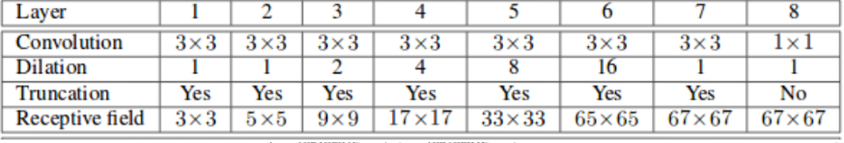
\includegraphics[width=\textwidth]{Context_dilation.png}
% where an .eps filename suffix will be assumed under latex,
% and a .pdf suffix will be assumed for pdflatex
\caption{Dilated contextual block. It is made up of multiple dilated convolution layers that slowly grow in dilation size to increase the receptive field size to 67x67. This contextual block is usually put at the end of the network in order to learn the context from the filters created from the previous network. As the layers increase the receptive field size increases as the dilation increases as well. Image is from \cite{Yu2016MultiScaleCA}.}
\label{fig_dilated_context}
\end{figure}
 
 One of the more popular models that has been adapted for dilated convolutions is VGG16. 
 VGG16 is a very widely used model for classification but has been adapted for many different tasks including semantic segmentation \cite{Simonyan15}. 
 VGG16 model is shown in figure ~\ref{fig_vgg16}. 
 VGG16 is originally used for classification which is why the output of the model is a 1x1. 
 For the task of semantic segmentation though we add zero padding before each layer to preserve the image size so the output is the same size as the input. 
 The first three pooling layers stride is changed to 1 in order to preserve the image size. 
 The last two pooling blocks are also removed and replaced by 3 dilation layers of dilation rate 1. 
 This makes the model simpler and easier for it to learn. 
 The contextual block is then put at the very end with zero padding in between each dilation layer \cite{Yu2016MultiScaleCA}. 
 This model proved to be too large to fit the MR images from this paper and so in this paper we modify the VGG model a bit by halving the filters used in every layer. 
 The full model we stack the halved filter VGG-16 model with the contextual block for the dilated convolutions coming afterwards. 
 We will refer to this model as the modified dilation VGG-16 model. 
 The total amount of parameters for this model is around 3 million. 
 This is significantly less than U-net and affects the results of the model. 
 
 \begin{figure}[tbh]
\centering
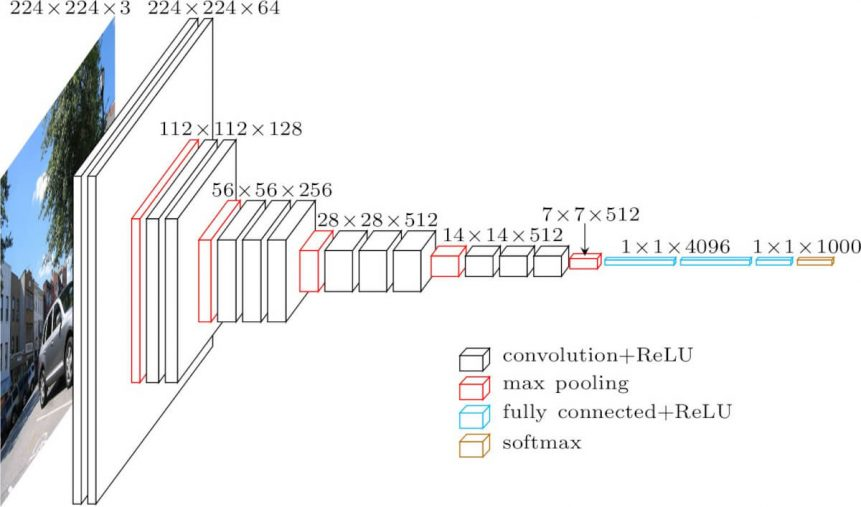
\includegraphics[width=\textwidth]{vgg16-neural-network.jpg}
% where an .eps filename suffix will be assumed under latex,
% and a .pdf suffix will be assumed for pdflatex
\caption{ This is the original VGG16 architecture. Its make convolutional and pooling layers make it a very robust model successfully used for classification. Image is from https://neurohive.io/en/popular-networks/vgg16/.}
\label{fig_vgg16}
\end{figure}
 
\subsection{U-net and dilation network}
Combined U-net with dilated convolutions is a relatively new idea, but has seen preliminary success in the segmentation of medical images \cite{10.1007/978-3-030-01449-0_16dilatedunet}, \cite{DBLP:journals/corr/abs-1805-10720}. 
The success of the U-net dilation networks comes from the idea of using the strength of both U-net and dilated convolutions together. 
The strength of U-net to find the relevant features combined with the strength of dilated convolutions to combine a multitude of features using the larger receptive field sizes. 
This combination can allow the network to learn about features that would previously be lost in pooling. 
The dilation contextual block was usually put at the lowest bottleneck of U-net to ensure that the most relevant features were combined \cite{10.1007/978-3-030-01449-0_16dilatedunet}. 
This is because the smallest bottleneck of Unet or when the downsampling stops is where the most important features for learning are and where we can get the most relevant features combined in many different ways according to the dilation. 
    
We implement this by taking our U-net architecture and applying the dilated contextual block within the bottleneck layer instead of convolutional layers. 
When the dilated contextual block is applied on the bottlneck layer the feature space size isn't that large because of all the downsampling layers. 
This helps to preserve space within the model and facilitate training.
In order to fully test this we implement the contextual layer with two to four downsampling layers.
We will refer to this model as the u-net dilation 2-4 downsampling model throughout this paper. 
The total amount of parameters for the 2-4 downsampling layers are around 9 million, 10 million, and 13 million respectively. 
This is much more compared to u-net which allows the u-net dilation models to learn much more complex connections. 
    
    
\section{Loss Functions}
    In the task of semantic segmentation there are two loss functions that are mainly used, dice coefficient and cross-entropy. 
    Loss functions are used to let the model know what to optimize for.
    There are pros and cons to both of the loss functions and each had their own fixes for their weaknesses. 
    It is not exactly clear which loss function is the best to use with some papers using to cross entropy \cite{DBLP:journals/corr/ChenPK0Y16} and most others using dice coefficient \cite{10.1007/978-3-030-01449-0_16dilatedunet}, \cite{DBLP:journals/corr/abs-1805-10720}. Some of the reasoning to use dice coefficient rather than cross entropy is that dice coefficient directly maximizes how we see the prediction visually. 
    This paper is mainly concerned with visually how the segmented regions look and so this paper will focus on that.
    
    
\subsection{Dice Similarity Coefficient}
    Dice coefficient (DSC) was first introduced as a simple spatial overlap measure \cite{10.2307/1932409dice}. 
    Dice Similarity coefficient became a very useful measure of spatial overlap which is very helpful in the task of semantic segmentation \cite{dice2004}. 
    Dice Coefficient can be calculated below where A and B are regions that need to be compared
\begin{equation}
 DSC = \frac{2*|A \cap B|}{|A| + |B|}\label{eq:dicescore} 
\end{equation}
    $|A|$ and $|B|$ represent the number of elements in each set. 
    If the regions in A and B directly match the the union of the two will give the total number of elements in the region. 
    The denominator will give the total number of elements in A and B which will match the numerator. 
    The max value of the dice score is one and the min value is zero when the union between the two sets is zero. 
    The negation of the calculation of the dice coefficient can be used as a loss function for the model to learn from. 
    Dice coefficent metric performs better with class imbalances because it is a ratio of the predicted and the ground truth. 
    Dice coefficient though is more unstable when training a model because the derivative of this function isn't easily calculated and blows up easier.
    
    One problem that arises when trying to train networks using the DSC is if there are slices of the volume that don't have ground truths associated for it then we can get a division by zero. 
    If the ground truth has no pixels in one particular slice then we would want the prediction to also have zero pixels predicted which gets us the zero in the denominator. 
    This is problematic for training because it is very hard for every region to be segmented to be in every slice in the MRI volume, especially if you want multiple regions segmented. 
    The solution for this is the add a smoothing factor to the DSC to prevent those cases. 
    In this case one is added the the numerator and the denominator of the fraction to calculate the DSC.
    
    \begin{equation}
 DSC = \frac{2*|A \cap B| + 1}{|A| + |B| + 1}\label{eq:dicescoreloss} 
\end{equation}
    By adding one to the numerator and denominator we change the calculation of the DSC a bit, but get rid of the division by zero case as well as keep the range of values from [0,1]. 
    This allows for the DSC to be used in training a model using backpropagation. 
    

\subsection{Cross-Entropy}
    Cross-entropy (CE) as a loss function has been used significantly in training models as it is simple and effective method to train models \cite{deBoer2005}. 
    Cross entropy can be calculated below where $M$ represents the total number of classes, $y$ represents the correct classification for $c$, and $p$ represents predicted probability it belongs to class c. 
\begin{equation}
 CE = -\sum_{c=1}^{M}{y_{c}log(p_{c})}  \label{eq:crossentropy} 
\end{equation}
    The min value of cross-entropy is zero where the model is able to predict with full confidence the correct class. 
    Cross-entropy punishes the predictions with the wrong label with high confidence the greatest as it had a higher significance on the loss function. 
    Cross entropy is also clearly defined in backpropogation unlike dice coefficient. 
    Cross-entropy though doesn't work well for class imbalances as it will give the larger classes priority over the smaller classes.
    This is a big deal for semantic segmentation because a lot of the time the regions that are needed to be segmented are small. 
